\section{Discussions et perspectives}
\subsection{Perspectives du workflow NGS pour la technologie MGI}

\subsubsection{Améliorations futures du pipeline NGS\_RG pour la technologie MGI}
Les pipelines de génération de fichiers de séquences est très spécifique à l'environement de gestion des projets de séquençage du Genoscope et du CNRGH, ainsi qu'à la base de données NGL. Celui pour la technologie MGI est inspiré du pipeline de l'autre technologie de séquençage \emph{short reads} (Illumina) déja en place, dont la finalité du pipline est le même, c'est à dire la prise en charge des données de séquençage en fin de séquençage et la mise à disposition des fichiers de séquences et des métriques d'évaluation.\\

La future amélioration du pipeline NGS\_RG\_MGI, consistera à la mise en place d'une étape suplémentaire pour les runs qui comporterons des \emph{mids}\footnote{un mid (\emph{molecular identifer}) est une séquence d'une dizaine de nucléotides ajoutés en aval du \emph{primer} du read \emph{forward} permettant de réaliser un second démultipléxage}. 
Un \emph{mid} est une séquence d'une dizaines de nucléotides ajoutés en amont du primer du read \emph{forward} (figure \ref{schema-mid}). Il s'agit d'un index suplémentaire qui permet lors du séquençage de déposer un nombres plus important d'échantillons différents sur une même piste d'une flowcell. 

\begin{figure}[H]
    \centering
    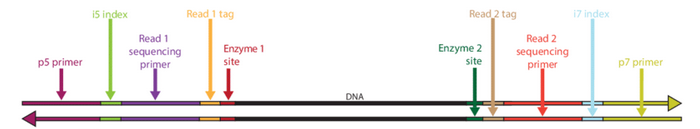
\includegraphics[width=0.8\textwidth]{img/schema-reads-index-mids.png}
    \caption{\footnotesize{Schéma représentant le vecteur à séquencer qui contient les index (i5 index et i7 index), les mids (Read 1 tag et Read 2 tag), les primers des index (p5 primer et p7 primer) et des reads (Read 1 sequencing primer et Read 2 sequencing primer), ainsi que l'ADN d'intérêt (en noir) et les sites enzymatiques permettant l'insertion de l'ADN d'intérêt dans le vecteur (Enzyme 1 site et Enzyme 2 site).}}
    \label{schema-mid}
\end{figure}

L'étape supplémentaire sera d'ajouter est un second démultipléxage en fonction de ces mids, qu'on appelle le démidage pour la création des readset et des fichiers de séquences.

\subsubsection{Développement du pipeline de contrôle qualité pour le technologie MGI}
Le pipeline de contrôle qualité des fichiers de séquences pour la technologie MGI, sera constitué de deux grande phases. La première consistera à réaliser un contrôle qualité des fichiers \og raw\fg{} (fichiers de séquences bruts), puis dans un second temps de réaliser un contôle qualité sur les fichiers \og clean\fg{} (fichiers de séquences néttoyés) ainsi que d'autres traitements sur les fichiers \og clean\fg{}.\\

Le pipeline devera prendre en charge automatiquement les fichiers dont les readset sont dans l'état \og IW-QC\fg{} dans NGL, qui représente les readset en attente de controle qualité. Celui-ci devera suivre le schéma de traitements et d'analyse (figure \ref{schema-workflow-ngsqc}) déja en place pour l'autre technologie de séquençage \emph{short reads} (Illumina). L'étape de nettoyage du \emph{PhiX} ne sera pas nécessaire pour la technologie MGI, puisque pour cette dernière il n'est pas utile d'ajouter ces séquences de contrôle.\\

\begin{minipage}{0.45\textwidth}
    \begin{figure}[H]
        \centering
        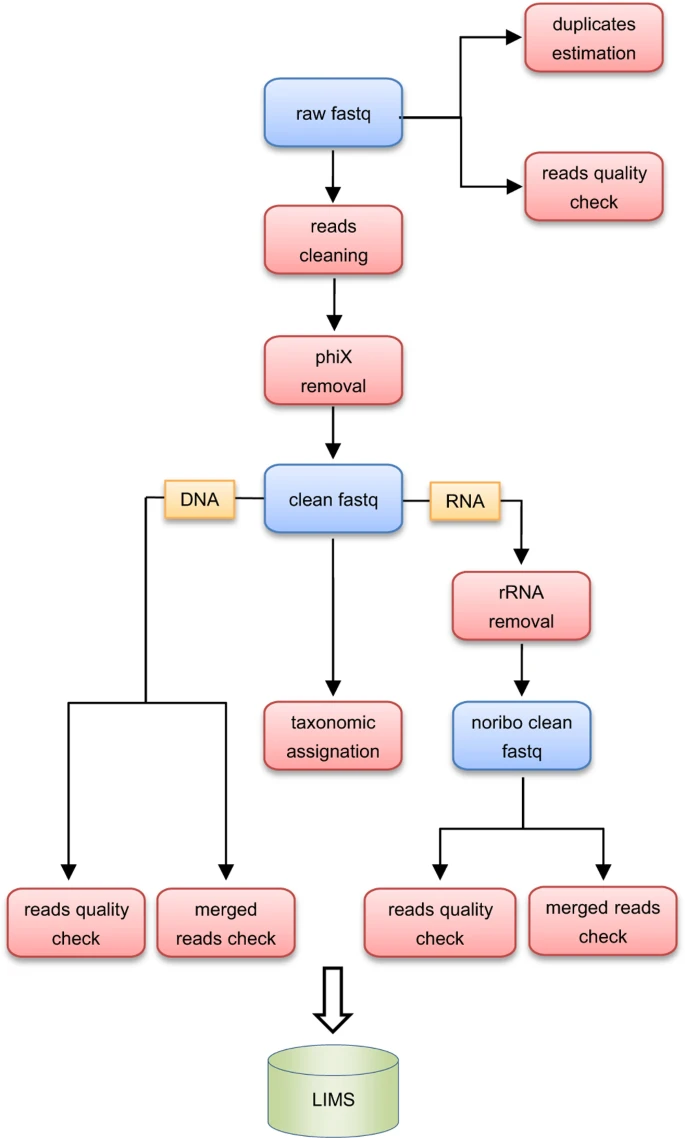
\includegraphics[width=1\textwidth]{img/schema-workflow-ngsqc.png}
        \caption{\footnotesize{Schéma de l'étape de renommage des fichiers FASTQ d'un readset}}
        \label{schema-workflow-ngsqc}
    \end{figure}
\end{minipage}
\hfill
\begin{minipage}{0.45\textwidth}

    Lors de la première phase on réalisera dans un premier temps un échantillonage de 20000 séquences par fichiers \og raw\fg{}. Cela permettera d'améliorer le temps d'execution du contrôle qualité, tout en ayant une grande représentativité de la qualité des séquences des fichiers \og raw\fg{}.\\

    Ensuite on réalisera le \og Trimming\fg{} (nettoyage des séquences) des fichiers \og raw\fg{}, avant de passer à la seconde phase du pipeline pour obtenir les fichiers \og clean\fg{}.\\

    Cette seconde phase commencera par un echantillonage de 20000 séquences par fichiers \og clean\fg{}, toujours dans l'optique d'améliorer le temps d'execution du contrôle quelité et des autres traitements sur les fichiers \og clean\fg{}.


\end{minipage}\\\\

Le Trimming consistera à retirer les séquences qui ont une qualité moyenne faible (inférieur à 20), les dernières bases des séquences qui ont une faible qualité (inférieur à 20) seront retirer de la séquence. Si il y a trop de bases inconnus dans la séquence celle-ci sera retirée, de même si dans la séquence ont retrouve 3 ou plus de bases inconnus successivement dans la séquence celle-ci sera coupé jusqu'à la fin de la séquence.\\


Les différentes étapes qui seront à réaliser pour la première phase sont :\\
\begin{itemize}
    \item[•] Réaliser le contrôle qualité des séquences des fichiers brut, avec l'outil fastx\_clean de l'extention \href{https://github.com/institut-de-genomique/fastxtend}{fastxend} de la suite \href{http://hannonlab.cshl.edu/fastx_toolkit/}{FASTX Toolkit} dévellopé par le Genoscope.
    \item[•] Réaliser l'estimation des duplicats des séquences des fichiers brut, avec l'outil fastx\_estimate\_duplicate de l'extenttion fastxend de la suite FASTX Toolkit dévellopé par le Genoscope.\\
\end{itemize}

Les différentes étapes qui seront à réaliser pour la seconde phase, une fois le Trimming effectué sont :\\
\begin{itemize}
    \item[•] Réaliser le contrôle qualité des séquences des fichiers clean, avec l'outil fastx\_clean.
    \item[•] Réaliser l'estimation des duplicats de séquences des fichier clean, avec l'outil fastx\_estmate\_duplicate.
    \item[•] Réaliser l'assignation taxonomique des séquences des fichiers clean, à l'aide du logiciel \href{https://ccb.jhu.edu/software/centrifuge/manual.shtml}{Centrifuge}.
    \item[•] Réaliser l'alignement des séquences des fichiers clean sur un génome de référence si celui-ci est disponible, à l'aide de l'outil \href{http://bio-bwa.sourceforge.net/bwa.shtml}{BWA}.
    \item[•] Réaliser le \og\emph{merging}\fg{} des séquences des reads \emph{foward} et \emph{reverse} pour les run \emph{pair end} (calcule du pourcentage de reads qui ont le read \emph{forward} et \emph{reverse} qui se chevauchent, calcule de la moyenne et médiane du nobre de bases qui ce chevauchent entre les 2 reads, \dots), à l'aide de l'outil fastx\_mergepairs de l'extention fastxend de la suite FASTX Toolkit développé par le Genoscope.\\
\end{itemize}

Une fois les étapes de la seconde phase réalisées, il sera nécessaire de réaliser la distribution des fichiers de séquences nettoyés dans leur répertoire final. Les fichiers raw seront alors effacés si ces derniers ont été archivé sur bande magnétique, et rendu indisponible pour les utilisateurs. L'objectif étant de permettre aux utilisateurs d'avoir les fichiers de séquences avec le meilleurs niveau de qualité possible.\\

Durant toutes les etapes du pipeline, on insert les métriques et graphiques obtenus au cours des différentes étapes du pipeline dans NGL\_BI. Ce qui permettera de réaliser la validation des readset ou non. L'intéraction entre le pipeline et la base de données est réalisée, comme pour le pipeline NGS\_RG\_MGI, par la librairie Perl (DBFactory) qui permet d'interagir avec NGL (cf. \ref{DBFactory} page \pageref{DBFactory}).\\

L'objectif est d'obtenir un pipeline de contrôle qualité opérationnel le plus rapidement possible, c'est pour cela que les outils utilisés seront les même que ceux utilisés pour le pipeline NGS\_QC\_Illumina. Néanmoins, les outils utilisés evolurons au fil du temps, avec les évalutaions d'outils pour les pipelines de contrôle qualité que je réaliserais au cours de l'année à suivre.

\subsection{Evaluation d'outils de contrôle qualité}
Les premiers outils à être évalués sont cutadapt et trimmomatic en vue d'un remplacement de fastx\_clean de FASTX Toolkit. Ce dernier est un logiciels mono-coeur contrairement à cutadapt et trimmomatic qui sont multi-coeurs. Le temps d'exécution entre ces logiciels sera le critère d'évaluation le plus important, néaimoins on prendra également en compte les différents fichiers de sortie (fichiers de statistiques, fichiers de séquences qui ne passe pas les filtres données \dots) pour l'évaluation et le remplacement de fastx\_clean.\\

Un potentiel successeur au logiciels d'assignation taxonomique Centrifuge devra egalement être effectuer, dans l'optique d'améliorer les pipelines de contrôle qualité. L'objectif est de trouver un logiciels dont les performance son équivalentes ou meilleurs, surtout au niveau du temps d'exécution, mais également au niveau de l'assignation taxonimique des séquences et des fichiers de sortie.